

\documentclass[table]{article}

\usepackage{graphicx}			% Use this package to include images
\usepackage{amsmath}			% A library of many standard math expressions
\usepackage[margin=0.75in, a4paper]{geometry}% Sets 1in margins. 
\usepackage{fancyhdr}			% Creates headers and footers
\usepackage{enumerate}          %These two package give custom labels to a list
\usepackage[shortlabels]{enumitem}
\usepackage{tikz}
\usepackage{float} % Add this in your preamble for using [H]
\usepackage{subcaption}
\usepackage{booktabs}
\usepackage{caption}
\usepackage[normalem]{ulem}
\useunder{\uline}{\ul}{}
\usepackage{circuitikz}
\usepackage{ragged2e} % Package for justification
\justifying

\graphicspath{{img/}}
\usetikzlibrary{shapes.geometric, arrows, positioning}

\def\mytitle{Homework 3}
\def\righthead{EEF205E}


\usepackage[T1]{fontenc}
\usepackage{lmodern}

%%%%%%%%%%%%%%%%%%%%%%%%%%%%%%%%%%%%%%%%%%%%%%%%%%%%%%%%
\pagestyle{fancy}
\fancyhead[l]{Rüzgar Erik}
\fancyhead[c]{\mytitle}
\fancyhead[r]{\righthead}
\fancyfoot[c]{\thepage}
\renewcommand{\headrulewidth}{0.2pt}
\setlength{\headheight}{15pt}
%%%%%%%%%%%%%%%%%%%%%%%%%%%%%%%%%%%%%%%%%%%%%%%%%%%%%%%%
\usepackage{parskip}
\setlength{\parindent}{0pt} % Disable paragraph indentation
%%%%%%%%%%%%%%%%%%%%%%%%%%%%%%%%%%%%%%%%%%%%%%%%%%%%%%%%


\usepackage{listings}
\usepackage{xcolor}
\usepackage{svg}

\lstdefinestyle{vhdlstyle}{
    language=VHDL,
    backgroundcolor=\color{white},
    basicstyle=\ttfamily,
    keywordstyle=\color{blue},
    commentstyle=\color{green},
    stringstyle=\color{red},
    numbers=left,
    numberstyle=\tiny\color{gray},
    stepnumber=1,
    numbersep=5pt,
    tabsize=2,
    showspaces=false,
    showstringspaces=false,
}



\usepackage{karnaugh-map}
\usetikzlibrary{calc}


\usepackage{hyperref}

\hypersetup{
  pdfauthor={Rüzgar Erik},
  pdftitle={\mytitle},
  pdfsubject={\righthead},
  pdfcreator={LaTeX},
  pdfproducer={Rüzgar Erik}
}






\begin{document}


\begin{titlepage}
    \begin{figure}[h] % Places the figure at the right
        \begin{flushright}
        
\includegraphics[width=0.3\textwidth]{logo_laci.png} % Change to your image name
            
        \end{flushright}
        \hfill
    \end{figure}

    \centering
    \vspace*{1in}
    
    \Huge
    \textbf{Introduction to Logic Design} \\
    \textbf{EEF205E} \\

    \vspace{0.5in}

    \Large
    \textbf{\mytitle} \\
    
    \vspace{0.5in}

    \large
    \textbf{Rüzgar Erik} \\
    \textbf{040240783} \\

    \vspace{0.5in}
    
    \Large
    Istanbul Technical University \\
    Faculty of Electrical and Electronics Engineering \\
    
    \vfill


\end{titlepage}



\section*{Part 1}

\begin{enumerate}
    \item Design a combinational circuit with three inputs, x, y and z, and three outputs, A, B, C.
    When the binary input is 0, 1, 2, or 3, the binary output is one greater than the input. When
    the binary input is 4, 5, 6, or 7, the binary output is two less than the input.

    Solution: The truth table for the given problem is shown below. \\

    
\begin{table}[H]
    \centering
    \caption{Truth Table for the given problem}
    \label{tab:enhanced-table}
    \resizebox{0.5\columnwidth}{!}{%
    \begin{tabular}{|c|c|c|c|c|c|c|c|}
    \hline
    \rowcolor[HTML]{CFE2F3} 
    \textbf{x} & \textbf{y} & \textbf{z} & \textbf{INPUT} & \textbf{A} & \textbf{B} & \textbf{C} & \textbf{OUTPUT} \\ \hline
    0          & 0          & 0          & 0              & 0          & 0          & 1          & 1              \\ \hline
    0          & 0          & 1          & 1              & 0          & 1          & 0          & 2              \\ \hline
    0          & 1          & 0          & 2              & 0          & 1          & 1          & 3              \\ \hline
    0          & 1          & 1          & 3              & 1          & 0          & 0          & 4              \\ \hline
    1          & 0          & 0          & 4              & 0          & 1          & 0          & 2              \\ \hline
    1          & 0          & 1          & 5              & 0          & 1          & 1          & 3              \\ \hline
    1          & 1          & 0          & 6              & 1          & 0          & 0          & 4              \\ \hline
    1          & 1          & 1          & 7              & 1          & 0          & 1          & 5              \\ \hline
    \end{tabular}%
    }
    \end{table}



Generating Kmaps For A, B, C outputs:


\begin{figure}[h]
    \centering
    % Subfigure for A output
    \begin{subfigure}{0.3\textwidth}
    \centering
    \begin{karnaugh-map}[4][2][1][$z$][$y$][$x$]
        \minterms{3,6,7}
        \maxterms{0,1,2,4,5}
        \implicant{3}{7}
        \implicant{7}{6}
    \end{karnaugh-map}
    \caption{Kmap for A output}
    \label{fig:kmapA}
    \end{subfigure}
    % Subfigure for B output
    \begin{subfigure}{0.3\textwidth}
    \centering
    \begin{karnaugh-map}[4][2][1][$z$][$y$][$x$]
        \minterms{1,2,4,5}
        \maxterms{0,3,6,7}
        \implicant{4}{5}
        \implicant{1}{5}
        \implicant{2}{2}
    \end{karnaugh-map}
    \caption{Kmap for B output}
    \label{fig:kmapB}
    \end{subfigure}
    % Subfigure for C output
    \begin{subfigure}{0.3\textwidth}
    \centering
    \begin{karnaugh-map}[4][2][1][$z$][$y$][$x$]
        \minterms{0,2,5,7}
        \maxterms{1,3,4,6}
        \implicantedge{0}{0}{2}{2}
        \implicant{5}{7}
    \end{karnaugh-map}
    \caption{Kmap for C output}
    \label{fig:kmapC}
    \end{subfigure}
    \caption{Karnaugh maps for outputs A, B, and C}
    \label{fig:kmapOverall}
    \end{figure}


Calculating the minimized expressions for A, B, C outputs:

\begin{align}
    A &= yz + xy \\
    B &= xy' + y'z + x'yz' \\
    C &= z' + xz
\end{align}


\newpage

\item A majority circuit is a combinational circuit whose output is equal to 1 if the input variables
have more 1’s than 0’s. The output is 0 otherwise. Design a 3-input majority circuit by
finding the circuit’s truth table, Boolean equation, and a logic diagram.


Solution: The truth table for the given problem is shown below. \\


\begin{table}[H]
    \centering
    \caption{Truth Table for the given problem}
    \label{tab:my-table}
    \resizebox{0.3\columnwidth}{!}{%
    \begin{tabular}{|c|c|c|c|c|}
    \hline
    \rowcolor[HTML]{CFE2F3} 
    \textbf{Index} & \textbf{x} & \textbf{y} & \textbf{z} & \textbf{Out} \\ \hline
    0              & 0          & 0          & 0          & 0            \\ \hline
    1              & 0          & 0          & 1          & 0            \\ \hline
    2              & 0          & 1          & 0          & 0            \\ \hline
    3              & 0          & 1          & 1          & 1            \\ \hline
    4              & 1          & 0          & 0          & 0            \\ \hline
    5              & 1          & 0          & 1          & 1            \\ \hline
    6              & 1          & 1          & 0          & 1            \\ \hline
    7              & 1          & 1          & 1          & 1            \\ \hline
    \end{tabular}%
    }
\end{table}


The kmap for the given problem is shown below:

\begin{figure}[H]
    \centering
    \begin{karnaugh-map}[4][2][1][$z$][$y$][$x$]
        \minterms{3,5,6,7}
        \maxterms{0,1,2,4}
        \implicant{3}{7}
        \implicant{5}{7}
        \implicant{7}{6}
    \end{karnaugh-map}
    \caption{Kmap for the majority circuit}
    \label{fig:majorityKmap}
\end{figure}

The minimized expression for the majority circuit is:

\begin{equation}
    Out = yz + xz + xy
\end{equation}


The logic diagram for the majority circuit is shown below:

\begin{figure}[H]
    \centering
    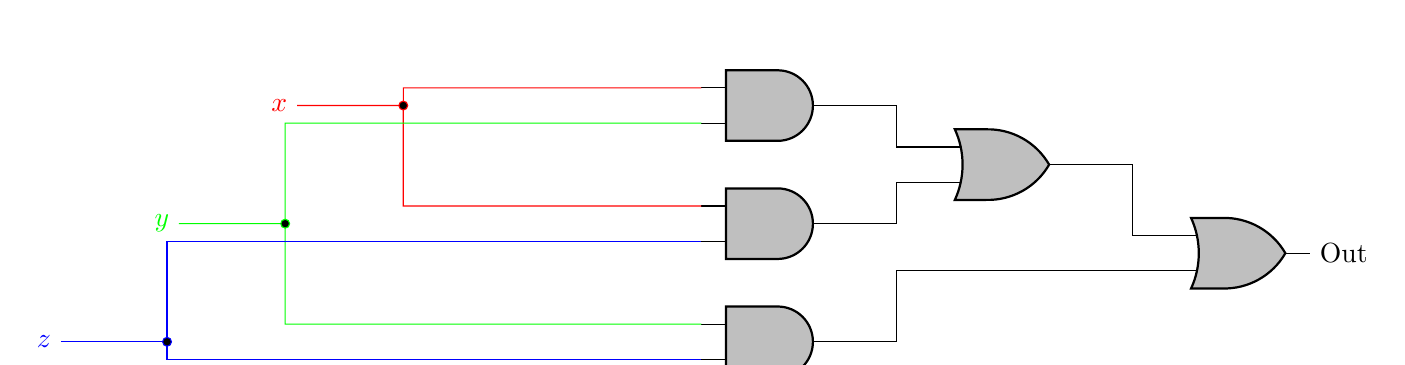
\begin{tikzpicture}[scale=1.5]
    \ctikzset{
        logic ports=ieee,
        logic ports/scale=0.8,
        logic ports/fill=lightgray
    }
    % Input points with staggered positions to prevent shorts
    \coordinate (x_in) at (-4,2) {};
    \coordinate (y_in) at (-5,1) {};
    \coordinate (z_in) at (-6,0) {};
    
    % Label inputs with colors
    \node[left, red] at (x_in) {$x$};
    \node[left, green] at (y_in) {$y$};
    \node[left, blue] at (z_in) {$z$};
    
    % First level AND gates
    \node[and port] (and1) at (0,2) {};
    \node[and port] (and2) at (0,1) {};
    \node[and port] (and3) at (0,0) {};
    
    % OR gates
    \node[or port] (or1) at (2,1.5) {};
    \node[or port] (or2) at (4,0.75) {};
    
    % Input connections with junction points and colors
    \draw[red] (x_in) -- ++(0.4,0) to[short,-*] ++(0.5,0) coordinate(x_junction)
        |- (and1.in 1) (x_junction) |- (and2.in 1);
    
    \draw[green] (y_in) -- ++(0.4,0) to[short,-*] ++(0.5,0) coordinate(y_junction)
        |- (and1.in 2) (y_junction) |- (and3.in 1);
    
    \draw[blue] (z_in) -- ++(0.4,0) to[short,-*] ++(0.5,0) coordinate(z_junction)
        |- (and2.in 2) (z_junction) |- (and3.in 2);
    
    % Connect AND gates to first OR gate
    \draw (and1.out) -- ++(0.5,0) |- (or1.in 1);
    \draw (and2.out) -- ++(0.5,0) |- (or1.in 2);
    
    % Connect first OR gate to second OR gate and third AND to second OR gate
    \draw (or1.out) -- ++(0.5,0) |- (or2.in 1);
    \draw (and3.out) -- ++(0.5,0) |- (or2.in 2);
    
    % Output label
    \node[right] at (or2.out) {$\text{Out}$};
    
    \end{tikzpicture}
    \caption{Logic diagram for the majority circuit}
    \end{figure}




\end{enumerate}

\newpage

\section*{Part 2}

\begin{enumerate}
    \item We will design a circuit called half adder (HA) which adds two 1-bit numbers, a, b and
    produces 2-bit output, c.

    \begin{enumerate}[label=(\alph*)]
        \item Draw the truth table of the circuit.
        
        Solution: The truth table for the given problem is shown below. \\

        \begin{table}[H]
            \centering
            \caption{Truth Table for the given problem (Part 2a)}
            \label{tab:part2a}
            \resizebox{0.3\columnwidth}{!}{%
            \begin{tabular}{|c|c|c|c|c|}
            \hline
            \rowcolor[HTML]{CFE2F3} 
            \textbf{a} & \textbf{b} & \textbf{Carry} & \textbf{Sum} \\ \hline
            0          & 0          & 0             & 0          \\ \hline
            0          & 1          & 0             & 1          \\ \hline
            1          & 0          & 0             & 1          \\ \hline
            1          & 1          & 1             & 0          \\ \hline
            \end{tabular}%
            }
        \end{table}

        \item Find the Boolean functions of each bit of the output.
        
        Solution: The Boolean functions for the given problem are shown below. 

        \begin{align}
            \text{Carry} &= ab \\
            \text{Sum} &= a \oplus b
        \end{align}

        It can be seen from the truth table that the carry bit is the AND of the inputs, and the sum bit is the XOR of the inputs.

        To obtain an XOR gate we can draw the Kmap for the sum bit:

        \begin{figure}[H]
            \centering
            \begin{karnaugh-map}[2][2][1][$b$][$a$]
                \minterms{1,2}
                \maxterms{0,3}
                \implicant{1}{1}
                \implicant{2}{2}
            \end{karnaugh-map}
            \caption{Kmap for the sum bit}
            \label{fig:sumKmap}
        \end{figure}

        The minimized expression for the sum bit is:

        \begin{equation}
            \text{Sum} = a'b + ab'
        \end{equation}

        Or we can simply use the XOR gate.

        \item Optimize the Boolean functions of each bit of the output.
        
        Solution: The optimized Boolean functions for the given problem are shown below.

        \begin{align}
            \text{Carry} &= ab \\
            \text{Sum} &= a \oplus b
        \end{align}

        The functions are already optimized.
        

        \item Draw the logic diagram of the circuit.
        
        Solution: The logic diagram for the given problem is shown below. \\
        \begin{figure}[H]
            \centering
            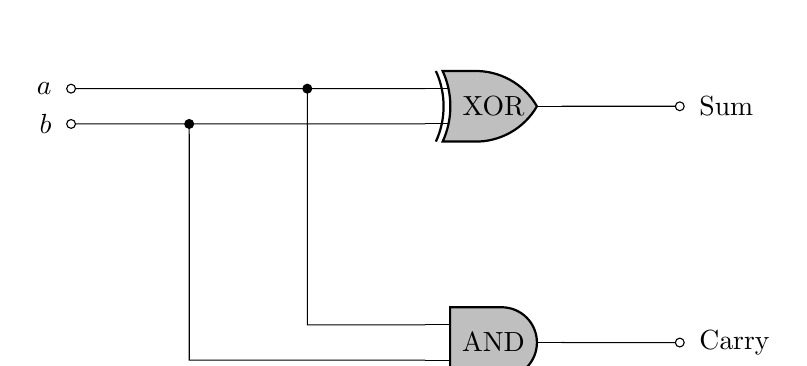
\begin{tikzpicture}[scale=1.5]
            \ctikzset{
                logic ports=ieee,
                logic ports/scale=0.8,
                logic ports/fill=lightgray
            }
        
            \draw
            (0,0)
            node[label=left:$a$] (a) {}
            to[short, o-] 
            (3,0)
            node[xor port, anchor=in 1] (carly) {XOR}
            (0,52 |- carly.in 2)
            node[label=left:$b$] (b) {}
            to[short, o-] 
            (carly.in 2)
            (carly.out)
            to[short, -o] 
            ++(1,0)
            node[label=right:$\text{Sum}$] {}
            (3,-2)
            node[and port, anchor=in 1] (percy) {AND}
            (percy.in 1)
             -- ++(-1,0)
            to[short, -*] (2,0)
            (percy.in 2)
            -- ++(-2,0)
            to[short, -*] (1,52 |- carly.in 2)
            (percy.out)
            to[short, -o] ++(1,0)
            node[label=right:$\text{Carry}$] {};

            \end{tikzpicture}
            \caption{Logic diagram for the half-adder circuit }
        \end{figure}
        
        \item Write the VHDL code of the logic diagrams by using “Dataflow modeling” method.
        
        Solution: The VHDL code for the given problem is shown below.

        \begin{center} % Center the entire code block
            \lstset{
          caption= half\_adder.vhd, 
          basicstyle=\footnotesize, frame=tb,
          xleftmargin=.2\textwidth, xrightmargin=.2\textwidth
        }
            \lstinputlisting[style=vhdlstyle]{code/half_adder.vhd}
        
        \end{center}


        \item Simulate the circuit that you have designed in 1.e. Prepare a simulation waveform for you
        report

        Solution: The simulation waveform for the given problem is shown below.

        \begin{figure}[H]
            \centering
            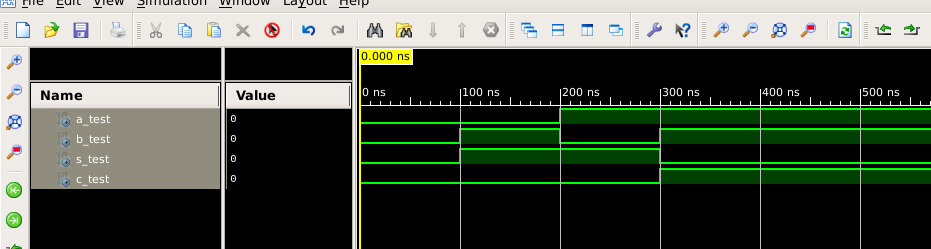
\includegraphics[width=0.8\textwidth]{ha_sim.png}
            \caption{Simulation waveform for the half-adder circuit}
            \label{fig:halfAdder}
        \end{figure}

        \item Produce the RTL schematic for the circuit that you have designed in 1.e.
        
        Solution: The RTL schematic for the given problem is shown below.

        \begin{figure}[H]
            \centering
            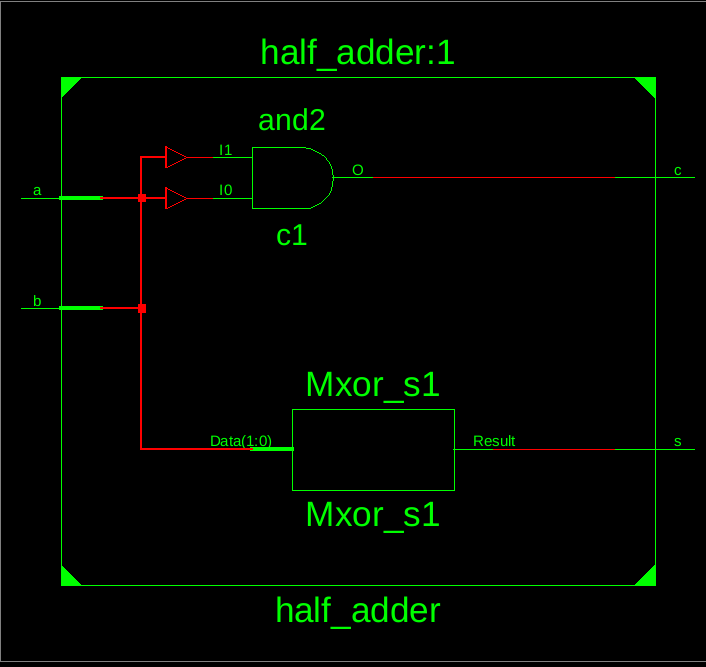
\includegraphics[width=0.8\textwidth]{ha_rtl.png}
            \caption{RTL schematic for the half-adder circuit}
            \label{fig:halfAdderRTL}
        \end{figure}

    \end{enumerate}
    
    \newpage


    \item We will design a circuit called full adder (FA) which adds three 1-bit numbers, a, b, c and
    produces 2-bit output, d.


    \begin{enumerate}
        \item Draw the truth table of the circuit.
        
        \begin{table}[H]
            \centering
            \caption{Truth Table for the given problem (Part 2.2.a)}
            \label{tab:part22a}
            \resizebox{0.4\columnwidth}{!}{%
            \begin{tabular}{|c|c|c|c|c|}
            \hline
            \rowcolor[HTML]{CFE2F3} 
            \textbf{a} & \textbf{b} & \textbf{Carry\_In} & \textbf{Carry\_Out} & \textbf{Sum} \\ \hline
            0 & 0 & 0 & 0     & 0   \\ \hline
            0 & 0 & 1 & 0     & 1   \\ \hline
            0 & 1 & 0 & 0     & 1   \\ \hline
            0 & 1 & 1 & 1     & 0   \\ \hline
            1 & 0 & 0 & 0     & 1   \\ \hline
            1 & 0 & 1 & 1     & 0   \\ \hline
            1 & 1 & 0 & 1     & 0   \\ \hline
            1 & 1 & 1 & 1     & 1   \\ \bottomrule
            \end{tabular}%
            }
        \end{table}

        \item Find the Boolean functions of each bit of the output.
        
        Solution: The Boolean functions for the given problem are shown below.

        \begin{align}
            \text{Carry\_Out} &= a'bc + ab'c + abc' + abc \\
            \text{Sum} &= a'b'c + a'bc' + ab'c' + abc
        \end{align}
        
        \item Optimize the Boolean functions of each bit of the output.
        
        Solution: The optimized Boolean functions for the given problem are shown below.

        Using Kmaps for the Carry\_Out and Sum bits:

        \begin{figure}[H]
            \centering
            \begin{subfigure}{0.5\textwidth}
                \centering
                \begin{karnaugh-map}[4][2][1][$c$][$b$][$a$]
                    \minterms{3,5,6,7}
                    \maxterms{0,1,2,4}
                    \implicant{3}{7}
                    \implicant{5}{7}
                    \implicant{7}{6}
                \end{karnaugh-map}
                \caption{Kmap for the Carry\_Out bit}
            \end{subfigure}
            \begin{subfigure}{0.5\textwidth}
                \centering
                \begin{karnaugh-map}[4][2][1][$c$][$b$][$a$]
                    \minterms{1,2,4,7}
                    \maxterms{0,3,5,6}

                    \implicant{4}{4}
                    \implicant{1}{1}
                    \implicant{2}{2}
                    \implicant{7}{7}

                \end{karnaugh-map}
                \caption{Kmap for the Sum bit}
            \end{subfigure}
            \caption{Karnaugh maps for Carry\_Out and Sum bits}
        \end{figure}
        The optimized expressions for the Carry\_Out and Sum bits are:

        \begin{align}
            \text{Carry\_Out} &= ac + bc + ab \\
            \text{Sum} &= ab'c' + a'b'c + abc + a'bc'
        \end{align}
    
        Also we can use the XOR and AND gates to implement the circuit.
    
        \begin{align}
            \text{Carry\_Out} &= ac + bc + ab \\
            \text{Sum} &= a \oplus b \oplus c
        \end{align}
    
        \item Draw the logic diagram of the circuit.
        
        Solution: The logic diagram for the given problem is shown below. 
    
        \begin{figure}[H]
            
            \centering
            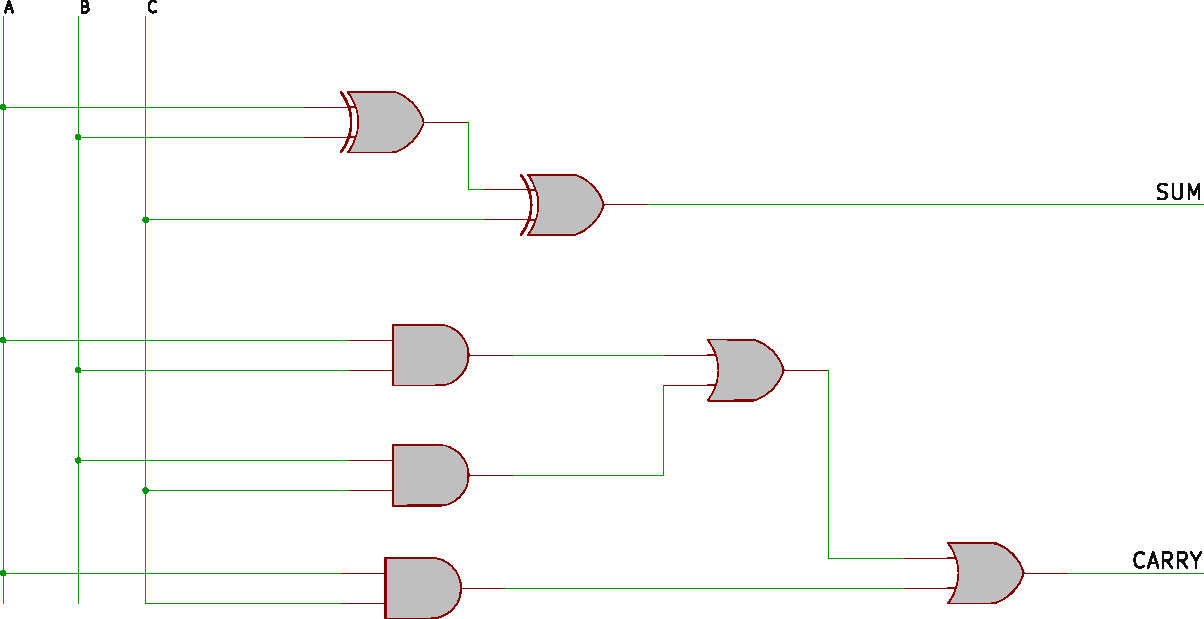
\includegraphics[width=0.8\textwidth]{g4.pdf}
            \caption{Logic diagram for the full-adder circuit}
            \label{fig:fullAdder}
        \end{figure}
    
        \item e. Write the VHDL code of the logic diagrams by using “Dataflow modeling”.
        
        Solution: The VHDL code for the given problem is shown below.

        
        \begin{center} % Center the entire code block
            \lstset{
          caption= full\_adder.vhd, 
          basicstyle=\footnotesize, frame=tb,
          xleftmargin=.2\textwidth, xrightmargin=.2\textwidth
        }
            \lstinputlisting[style=vhdlstyle]{code/full_adder.vhd}
        
        \end{center}

        \item Simulate the circuit that you have designed in 2.e. Prepare a simulation waveform for your report.
        
        Solution: The simulation waveform for the given problem is shown below.

        \begin{figure}[H]
            \centering
            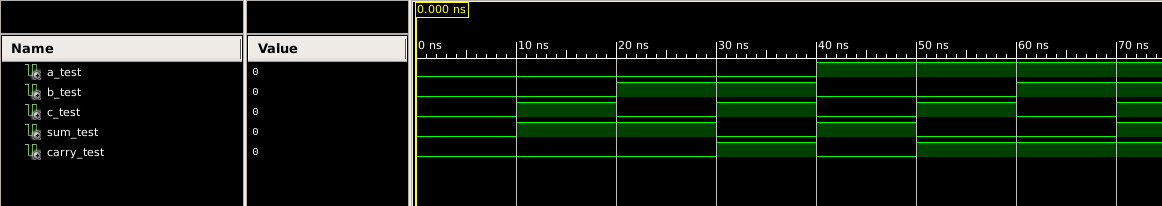
\includegraphics[width=0.8\textwidth]{fa_sim.png}
            \caption{Simulation waveform for the full-adder circuit}
            \label{fig:fullAdderSim}
        \end{figure}

        
        \item Produce the RTL schematic for the circuit that you have designed in 2.e.
        
        Solution: The RTL schematic for the given problem is shown below.

        \begin{figure}[H]
            \centering
            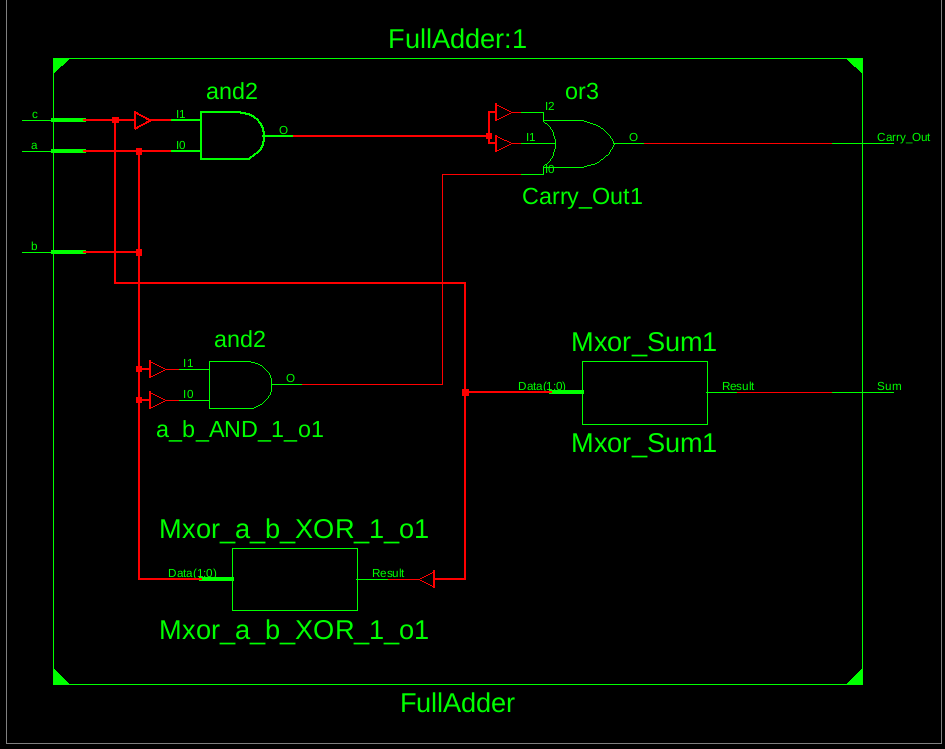
\includegraphics[width=0.4\textwidth]{fa_rtl.png}
            \caption{RTL schematic for the full-adder circuit}
            \label{fig:fullAdderRTL}
        \end{figure}


    
    \end{enumerate}



    \item We will design a circuit called ripple carry adder (RCA) which adds two 4-bit positive
    integers, A, B and produces 5-bit output, C.



    \begin{enumerate}[label=(\alph*)]
        \item Draw the logic diagram of the circuit by using one HA and 4 FAs.
    
        
        \begin{figure}[H]

            \centering
            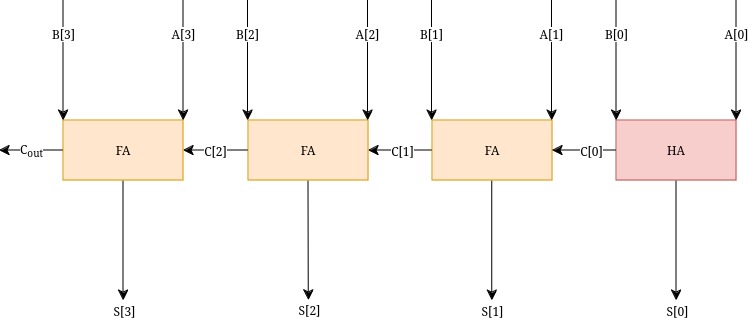
\includegraphics[width=0.8\textwidth]{rca.png}
            \caption{Logic diagram for the ripple carry adder circuit}
            \label{fig:rca}

                
            
        \end{figure}

        \newpage"


        \item Write the VHDL code of the logic diagrams by using “Structural modeling”

        Solution: The VHDL code for the given problem is shown below.

        \begin{center} % Center the entire code block
            \lstset{
          caption= ripple\_carry\_adder.vhd, 
          basicstyle=\footnotesize, frame=tb,
          xleftmargin=.2\textwidth, xrightmargin=.2\textwidth
        }
            \lstinputlisting[style=vhdlstyle]{code/rca.vhd}
        \end{center}

        \item Produce the RTL schematic for the circuit that you have designed in 3.b.
        
        Solution: The RTL schematic for the given problem is shown below.

        \begin{figure}[H]
            \centering
            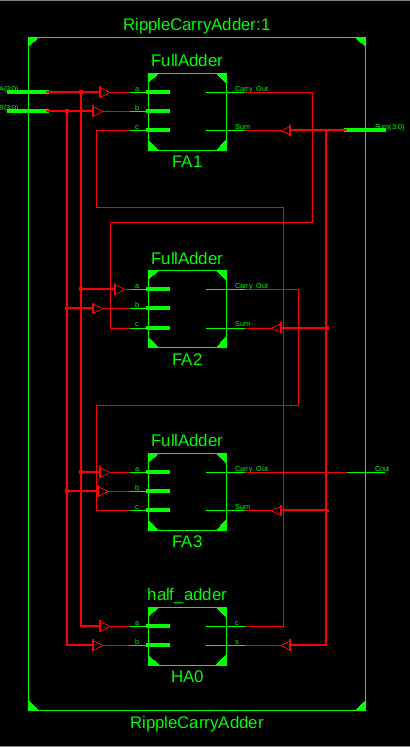
\includegraphics[width=0.3\textwidth]{rca_rtl.png}
            \caption{RTL schematic for the ripple carry adder circuit}
            \label{fig:rcaRTL}
        \end{figure}

        \newpage

        \item Simulate the circuit that you have designed in 3.b.
        
        Solution: The simulation waveform for the given problem is shown below.

        \begin{figure}[H]
            \centering
            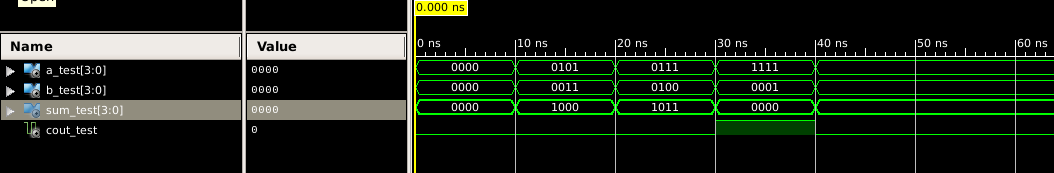
\includegraphics[width=\textwidth]{rca_sim.png}
            \caption{Simulation waveform for the ripple carry adder circuit}
            \label{fig:rcaSim}
        \end{figure}


    \end{enumerate}





    
\end{enumerate}





\end{document}